\section{Videojuegos desarrollados para la validación del sistema}
\label{sec:videojuegosDesarrollados}

Teniendo en cuenta los resultados obtenidos del modelo y todas las pruebas anteriores, se decidió trabajar con tan solo dos predicciones: mano derecha (\textit{right\_hand}) y mano izquierda (\textit{left\_hand}). Por ello, los juegos propuestos para el experimento debían tener como máximo dos controles.

Con esto en mente, se plantearon dos juegos que permitían poner a prueba la precisión y el tiempo de respuesta del sistema, además de la experiencia del usuario: \textit{wave runner} y \textit{project arrows}.

Para no perder tiempo extra en la implementación de los juegos, se decidió diseñarlos y pedir a un \textit{LLM}, por medio de un \textit{prompt} detallado, que proporcionara la implementación. Una vez generada, se revisó el código, se comprobó que cumplían todos los requerimientos y se hicieron algunos ajustes manuales.

\subsection{\textit{Endless Wave Runner}}
\label{subsec:endless_wave_runner}

Para el diseño de este juego se tomó como referencia la nave \textit{``wave''} del juego \textit{Geometry Dash}, de ahí el nombre. En la versión del \textit{Geometry Dash}, la nave avanza automáticamente de izquierda a derecha (realmente la nave permanece estática y es el escenario el que se mueve para dar la sensación de avance) y el jugador controla si se mueve en diagonal hacia arriba o hacia abajo, cambiando entre las dos opciones con una pulsación en la pantalla. El objetivo del juego es avanzar sin que la nave se choque, hasta terminar la fase (véase Figura~\ref{fig:wave_runner}). 

A diferencia del original, en esta versión el jugador avanza automáticamente de abajo hacia arriba, puede controlar si moverse en diagonal hacia la izquierda o hacia la derecha y la pantalla es ``infinita'' (haciendo que el objetivo sea aguantar lo máximo posible). Se consideró apropiado este juego debido a su simplicidad de controles y jugabilidad: el usuario tiene una tarea clara y sencilla que puede controlar con lo que ofrece el sistema de forma intuitiva. 

A la hora de diseñar el juego se tuvo en cuenta que este fuera configurable, para adaptar las velocidades y la dificultad a las limitaciones del casco EEG y del propio sistema. Se puede adaptar fácilmente, con tan solo cambiar los atributos de la clase: la velocidad en ambos ejes, la generación de obstáculos, el ancho inicial entre obstáculos, la distancia mínima entre obstáculos, el aumento de velocidad con el tiempo, la disminución del ancho del ``túnel'' (ancho entre obstáculos) y el \textit{respawn} automático, entre otros.

Como se ha mencionado anteriormente, se hizo uso de un \textit{LLM} para la implementación, concretamente Gemini\footnote{\url{https://gemini.google.com}}. El \textit{prompt} utilizado para la generación fue el siguiente:

\begingroup % 1. Abrimos el grupo local

% 2. Restauramos los valores estándar de LaTeX solo para esta zona
\tolerance=200
\hbadness=1000
\hyphenpenalty=50
\exhyphenpenalty=50
\emergencystretch=0pt

\begin{lstlisting}[
    breaklines=true,
    breakatwhitespace=true,
    basicstyle=\ttfamily\small,
    frame=single,
    columns=fullflexible,
    keepspaces=true,
    breakindent=0pt
]
Quiero que me hagas un juego basándote en la flecha del geometry dash. En el geometry dash existe un vehículo que es una flecha, este solo puede ir en diagonal hacia arriba derecha o hacia abajo derecha y cada vez q se pulsa en la pantalla cambia entre las dos opciones. Vamos a hacer una modificación a este vehículo para convertirlo en un juego nuevo y aislado:

En vez de avanzar de izquierda a derecha, nuestra flecha avanzará de abajo a arriba. De forma que la flecha tendrá dos opciones: ir hacia arriba izquierda en diagonal o hacia arriba derecha en diagonal. Y el cambio de los controles se hará mediante las flechas: al pulsar la flecha izquierda, nuestra flecha nave apuntará y se moverá hacia arriba izquierda; y al pulsar la flecha derecha nuestra nave apuntará y se moverá hacia arriba derecha. Debes añadir más funcionalidades para hacer pruebas: si se pulsa la flecha de arriba, nuestra flecha nave deberá apuntar directamente hacia arriba recto. Debe de haber una constante en el script q me permita activar/desactivar los obstáculos, si se generan obstáculos habrá a la izquierda y a la derecha de la pantalla pinchos sobresaliendo de distintos tamaños, algunos muy grandes, otros más pequeños (igual q en las zonas del geometry dash q se juegan con esta nave), si el jugador toca un obstáculo, pierde; en caso de q los obstáculos estén desactivados, la única forma de perder será saliéndose de la pantalla por los laterales (izquierdo y derecho). 
Deben existir constantes en el script para modificar la velocidad del juego, el avance por cada tick de la nave, el tiempo q pasa entre ``tick'' y ``tick'', etc. El avance de la nave debe de ser similar a un scroll, la nave realmente se quedará estática en su coordenada y, solo modificará su coordenada en x y su rotación, y será el propio mapa (el fondo (con algún dibujo que no maree para ver q avanza el juego) y, en caso de q los haya, los obstáculos) el que baje a la velocidad determinada por las variables. También deberá haber unas constantes para controlar la ``dificultad'', de forma q si se generan obstáculos, estos podrán dejar más o menos espacio para que el jugador maniobre en base a esa dificultad. Tema puntos: elige la forma q quieras de contarlos pero q haya puntos y q cuanto más tiempo sobrevivas, más puntos tengas. Debe también existir una constante que determine si hay ``respawn automático'' o no, si lo hay, la flecha al chocarse deberá reposicionarse en el ``lugar más seguro'' dentro de su misma coordenada y, dejando la mayor cantidad de hueco tanto a la izquierda como a la derecha sin q haya obstaculo; sin embargo si no hay respawn automático, el juego terminará, pondrá una pantalla ``game over'' y le indicará los puntos al jugador, además de una opción de volver a jugar con la tecla ``esc''. Por último, deberán existir otras constantes q determinen si el juego va a ir aumentando su dificultad o no: una constante q determine si se va a ir incrementando la velocidad, otra que diga cuanto se aumenta cada vez, y otra que determine cada cuanto se aumenta; otra que determine si se va a ir disminuyendo el espacio que hay para pasar entre los obstáculos, otra que determine cuánto disminuye cada vez y otra que determine cada cuánto se disminuye. 

Notas adicionales: Los obstáculos y el fondo deben de ir a la misma velocidad.

Todas las constantes definidas deberán tener un nombre significativo para que las pueda entender sin ninguna explicación a parte. También deberás explicar con un breve comentario al principio de cada función q hace la misma y, si es muy compleja, detallar de forma más detallada q algoritmo sigue para q podamos interpretarlo.

IMPORTANTE: siempre debe de haber un hueco lo suficientemente grande como para que la nave pase, el juego debe de ser posible de jugar, no puede haber en ningún momento una barrera que sea todo obstáculo ni dejar tan poco espacio que el jugador no pueda maniobrar.

En python con pygame. El juego debe estar contenido en una clase llamada EndlessWaveRunner, que se pueda utilizar desde fuera para llamar al juego.
\end{lstlisting}

\endgroup

\begin{figure}[h]
    \centering
    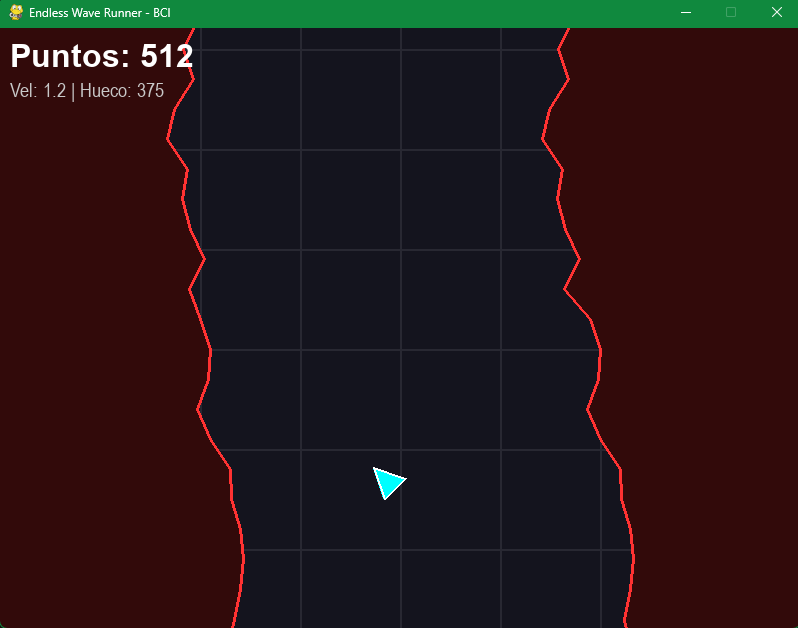
\includegraphics[width=0.7\textwidth]{Imagenes/Bitmap/Wave_runner.png}
    \caption{Visualización gráfica en ventana del juego Endless Wave Runner.}
    \label{fig:wave_runner}
\end{figure}


\subsection{\textit{Project Arrows}}
\label{subsec:project_arrows}

La inspiración para este juego fue \textit{``Project Rhombus''}, de \textit{Steam}. En el orignial, el jugador controla un rombo situado en mitad de la pantalla, este rombo tiene una flecha en su interior que apunta hacia arriba, abajo, izquierda o derecha de forma excluyente. Con las cuatro flechas del teclado, se controla hacia dónde apunta la flecha del rombo. A medida que avanza el juego, aparecen flechas por una de las cuatro direcciones posibles en el borde de la pantalla y avanzan hacia el centro. El objetivo de el jugador es defenderse, apuntando la flecha del rombo hacia la flecha enemiga que le vaya a alcanzar, si una flecha enemiga llega al rombo y este no está apuntando hacia ella, el jugador pierde (véase Figura~\ref{fig:project_arrows}).

En \textit{``Project Arrows''} se ha adaptado al sistema desarrollado quitando los controles de arriba y abajo, dejando únicamente izquierda y derecha. Se planteó este juego por los mismos motivos que el anterior.

Al igual que el anterior juego, se contempló que este fuera configurable y adaptable al sistema. Pudiendo modificar atributos como: la velocidad de las flechas enemigas, el tiempo de aparición de las mismas, el aumento de velocidad de estas, la posibilidad de reiniciar el juego automáticamente al morir\dots

Se contempló la posibilidad de añadir un tipo de flecha especial que cambia de lado a mitad de camino, se llegó a implementar pero finalmente se descartó por resultar demasiado complicado.

El \textit{prompt} utilizado para la generación mediante el \textit{LLM} Gemini\footnote{\url{https://gemini.google.com}} fue:

\begingroup % 1. Abrimos el grupo local

% 2. Restauramos los valores estándar de LaTeX solo para esta zona
\tolerance=200
\hbadness=1000
\hyphenpenalty=50
\exhyphenpenalty=50
\emergencystretch=0pt

\begin{lstlisting}[
    breaklines=true,
    breakatwhitespace=true,
    basicstyle=\ttfamily\small,
    frame=single,
    columns=fullflexible,
    keepspaces=true,
    breakindent=0pt
]
Quiero un juego que se base en el project rhombus, en caso de que no sepas cómo funciona te hago un resumen: en el centro está el ``personaje'' jugable, es una flecha que apunta arriba, abajo, a la izquierda O a la derecha (solo a una de esas 4 a la vez). Tiene música de fondo para acompañar los ritmos y van llegando flechas de esos 4 lados (desde fuera de la pantalla hacia adentro), si te toca una flecha y estás ``mirando'' (apuntando con tu personaje flecha) a otro lado, esta te mata y pierdes. El objetivo del juego es aguantar lo máximo posible y la puntuación se mide en segundos de la forma: 00.00 (siendo la parte decimal fracciones de un segundo). Ahora, quiero que realicemos una modificación para hacer un juego jugable con tan solo dos flechas (la izquierda y la derecha), lo q debes hacer es replicar el juego, hacer q solo podamos ``apuntar'' hacia la derecha o hacia la izquierda y que las flechas ``a bloquear'' también vengan únicamente de esos dos lados (desde fuera de la pantalla hacia adentro). Vamos a entrar en varios detalles importantes q debes añadir/controlar: debe haber constantes para controlar distintos aspectos del juego: una constante para controlar la velocidad de las flechas que vienen, otra para indicar si se va a ir aumentando esa velocidad con el paso del tiempo, otra que indique cuánto aumenta la velocidad por cada 0.01s en caso de que la de aumento sea True, otra constante para controlar si se generan flechas ``invertidas'' o no (en caso negativo solo se generarán flechas normales, que apuntan hacia el centro desde el principio).

Nota: de normal las flechas que vienen, apuntan hacia el centro (te apuntan ``a ti'' como jugador), sin embargo pueden existir flechas ``invertidas'', estas son flechas que vienen dadas la vuelta (por ejemplo, si vienen de el lado derecho, avanzan hacia el izquierdo pq quieren ir al centro pero apuntan hacia la derecha, van ``al revés'') estas, cuando están relativamente cerca del jugador, cambian de lado (si estaba en la izquierda, se mueve a la derecha y vice versa), haciendo q ahora la flecha apunte hacia el centro, y avanzan igualmente hacia el centro. son flechas diseñadas para confundir, son de otro color distintivo para verlas más fácil y no son muy complicadas de tratar dependiendo de la velocidad de las flechas. Importante para la jugabilidad y que el jugador no se pierda: las flechas invertidas deben cambiar de lado a una distancia prudencial y de una forma VISUAL (no quiero que se teletransporten, quiero que se desplacen visualmente, dejando tiempo de reacción, de un lado a otro) para que le jugador no las pierda de vista, y deben de mantener su color distintivo aunq ahora estén donde deban estar. 

si el jugador pulsa esc, el juego deberá pausarse y marcar en una pantalla que el juego está pausado, cuanto tiempo lleva sobrevivido hasta ahora el jugador y ``esc para continuar''. Si el jugador muere, dependerá de una constante si se reinicia la puntuación a 0 y se sigue con el juego (respawn automático = True) o si se para la ejecución, se cambia a una pantalla de game over, con el tiempo sobrevivido y un ``esc para reiniciar''

Notas adicionales: importante q la estética sea agradable. 

En python con pygame. El juego debe estar contenido en una clase llamada ProjectArrows, que se pueda utilizar desde fuera para llamar al juego.
\end{lstlisting}

\endgroup

\begin{figure}[h]
    \centering
    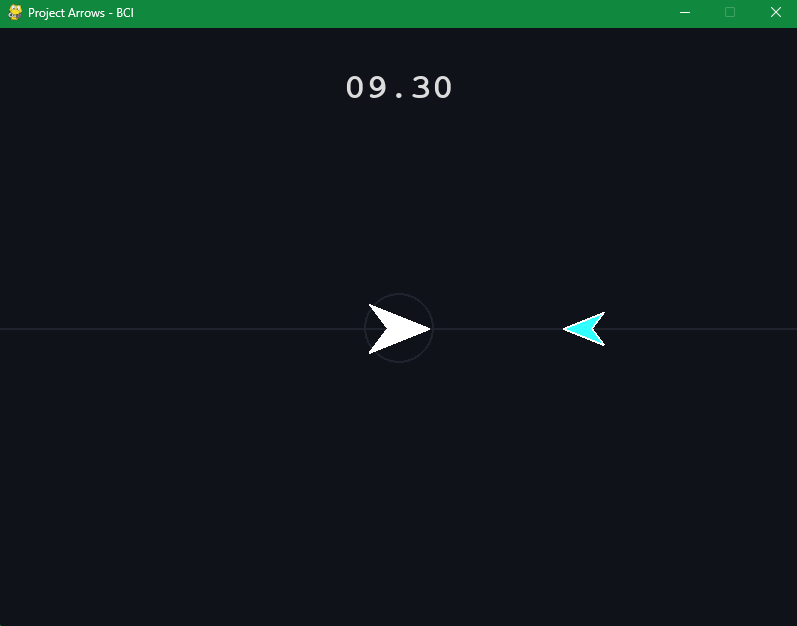
\includegraphics[width=0.7\textwidth]{Imagenes/Bitmap/Project_arrows.png}
    \caption{Visualización gráfica en ventana del juego Project Arrows.}
    \label{fig:project_arrows}
\end{figure}

Además de los juegos definidos, se diseñó un módulo de feedback visual (\textit{dualArrowComponent}) diseñado para tener una referencia de la destreza del usuario y de la latencia del sistema. 

\subsection{\textit{Benchmark} visual}
\label{subsec:benchmark_visual}

Dicho componente, al ejecutarse muestra una ventana en negro con dos flechas, una apuntando hacia la izquierda y la otra hacia la derecha. Está diseñado de forma que se puede cambiar el comportamiento con tan solo llamar a una función o a otra. Sin embargo, las funciones que nos interesan son las que permiten la funcionalidad que se mostrará en las pruebas que realizaremos más adelante (véase Figura~\ref{fig:benchmark_visual}). 

Cada flecha actúa como un contenedor, si llega una predicción se comprueba que el contenedor opuesto esté vacío: en caso de que lo esté, se suma un valor definido (\texttt{self.step}) al contenedor correspondiente a la predicción; en caso contrario, se le resta el doble de la cantidad que se hubiera sumado (\texttt{self.step * 2}). Por otro lado, en caso de que reciba \textit{``rest''}, se llamará a otra función que simplemente resta la misma cantidad (\texttt{self.step}) al contenedor que no esté vacío (en caso de que alguno de los dos tenga contenido). De esta forma, solo podrá rellenarse parcial o totalmente un contenedor a la vez, mientras el otro se mantiene vacío.

La implementación, de la misma forma que con los juegos, se realizó utilizando un \textit{LLM} (Gemini\footnote{\url{https://gemini.google.com}}). Se le proporcionó el siguiente \textit{prompt}:

\begingroup % 1. Abrimos el grupo local

% 2. Restauramos los valores estándar de LaTeX solo para esta zona
\tolerance=200
\hbadness=1000
\hyphenpenalty=50
\exhyphenpenalty=50
\emergencystretch=0pt

\begin{lstlisting}[
    breaklines=true,
    breakatwhitespace=true,
    basicstyle=\ttfamily\small,
    frame=single,
    columns=fullflexible,
    keepspaces=true,
    breakindent=0pt
]
Quiero hacer un script en python que actúe de componente, se pueda importar desde otros scripts e interactuar con este. La funcionalidad del script debe ser la siguiente: cuando se ejecute debe de abrirse una ventana con pygame que muestre con fondo negro, dos flechas de color azul oscuro (agradable a la vista) vacías, es decir solo debe de mostrar el contorno. las flechas deben de estar dispuestas una al lado de la otra, centradas de altura, la de la izquierda debe de apuntar hacia la izquierda, dejar un hueco no muy grande pero estético y debe de disponerse la otra flecha apuntando a la derecha. Ahora bien, eso nada más iniciarlo, pero el ``relleno'' de las flechas debe de ser en base a un porcentaje que el script debe de tener dentro del objeto como atributo de inicialización, la flecha izquierda tendrá un porcentaje y la derecha otro, así que dos variables. si el porcentaje de la izquierda es 0, la flecha izquierda debe de estar vacía excepto el contorno, si el porcentaje es un 50% debe de estar llena hasta la mitad, si es 100% debe de estar llena por completo, si es un porcentaje más raro y preciso como 64% la flecha deberá de estar rellena un 64%; lo mismo para la flecha derecha pero rellenándose en el sentido contrario. Las flechas se rellenarán desde el centro hacia fuera, es decir si ambas tienen un 1%, será la parte más cercana al centro la que se verá un poco rellena, si están al 70% será la parte más cercana al centro (el 70% de la flecha) la que se rellenará, y el otro 30% más lejano se quedará vacío excepto por el borde. El relleno debe de ser color azul también pero algo más claro y brillante (igualmente que sea agradable a la vista). y el objeto dentro del script debe de tener funciones para poder cambiar el valor de ambos porcentajes de forma independiente o a la vez, al igual que debe de tener una forma de resetear el objeto (poniendo ambos porcentajes a 0) y de consultar los porcentajes de las flechas. El color quiero poder cambiarlo yo manualmente en el código así que ponme claro dónde se define, y el tamaño de ventana debe de ser no muy grande, y modificable, de forma que si se ajusta el tamaño de la ventana las flechas ajusten su tamaño en proporción de forma acorde y sigan centradas de altura y bien dispuestas (dejando un hueco entre ellas en el medio) de forma correcta.
\end{lstlisting}

\endgroup % 4. Cerramos el grupo. A partir de aquí, vuelve tu justificado sin guiones.



Partiendo de la base que generó el \textit{LLM}, fue necesario hacer una pequeña modificación para hacer las flechas completamente simétricas y se implementaron a mano los métodos descritos en el párrafo anterior al prompt.

\begin{figure}[h]
    \centering
    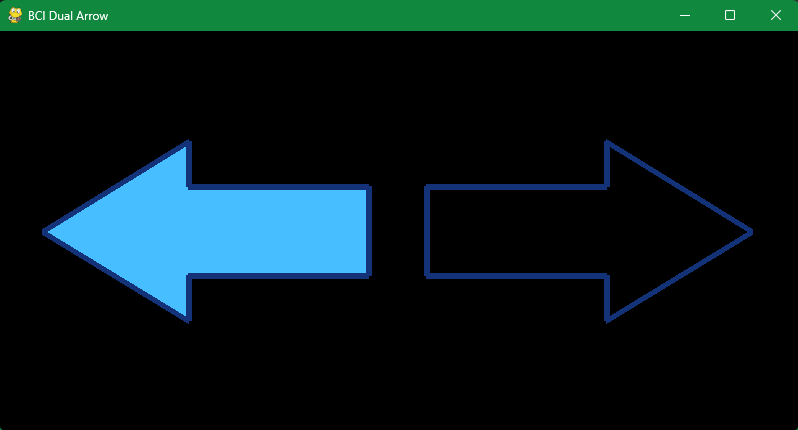
\includegraphics[width=0.7\textwidth]{Imagenes/Bitmap/Dual_arrow.png}
    \caption{Visualización gráfica en ventana del \textit{benchmark} de doble flecha.}
    \label{fig:benchmark_visual}
\end{figure}